\documentclass[conference]{IEEEtran}
\IEEEoverridecommandlockouts
\usepackage{cite}
\usepackage{amsmath,amssymb,amsfonts}
\usepackage{algorithmic}
\usepackage{algorithm}
\usepackage{graphicx}
\usepackage{textcomp}
\usepackage{xcolor}
\usepackage{booktabs}
\usepackage{multirow}
\usepackage{array}
\usepackage{url}
\usepackage{tikz}
\usetikzlibrary{positioning,arrows.meta,fit,calc}
\def\BibTeX{{\rm B\kern-.05em{\sc i\kern-.025em b}\kern-.08em
    T\kern-.1667em\lower.7ex\hbox{E}\kern-.125emX}}
\newcommand{\todo}[1]{\textcolor{red}{\textbf{[#1]}}}

\begin{document}

\title{Explainability-Aware Synthetic Oversampling for Imbalanced Tabular Classification: A Leakage-Free Benchmark of SHAP-Guided SMOTE Variants}

\author{
\IEEEauthorblockN{Prof. Gopal Deshmukh}
\IEEEauthorblockA{\textit{Dept. of Computer Engineering} \\
\textit{Vishwakarma Institute of Technology}\\
Pune, India \\
gopal.deshmukh@vit.edu}
\and
\IEEEauthorblockN{Rachit Ingole}
\IEEEauthorblockA{\textit{Dept. of Computer Engineering} \\
\textit{Vishwakarma Institute of Technology}\\
Pune, India \\
rachit.ingole241@vit.edu}
\and
\IEEEauthorblockN{Harshal Jaiswal}
\IEEEauthorblockA{\textit{Dept. of Computer Engineering} \\
\textit{Vishwakarma Institute of Technology}\\
Pune, India \\
harshal.jaiswal241@vit.edu}
\and
\IEEEauthorblockN{Hasan Rupawalla}
\IEEEauthorblockA{\textit{Dept. of Computer Engineering} \\
\textit{Vishwakarma Institute of Technology}\\
Pune, India \\
hasan.rupawalla24@vit.edu}
\and
\IEEEauthorblockN{Pranav Jagtap}
\IEEEauthorblockA{\textit{Dept. of Computer Engineering} \\
\textit{Vishwakarma Institute of Technology}\\
Pune, India \\
pranav.jagtap24@vit.edu}
}

\maketitle

\begin{abstract}
Synthetic minority over-sampling (SMOTE) generates new minority samples by linearly interpolating between nearest neighbours, equally weighing all features (informative or not). Explainability methods such as SHAP generally are applied only after model training, with its inclusion within data-balancing stage comparatively unexplored. This paper proposes and evaluates two Explainability aware oversamplers: SHAP-Filtered SMOTE (restricts neighbor search to a subspace selected by mean absolute SHAP values (MASV)) and SHAP-Weighted SMOTE (replaces the Euclidean metric with a MASV-weighted metric). In this paper we compare against seven baseline approaches (no balancing, random oversampling, SMOTE, Borderline-SMOTE, ADASYN, SMOTE-ENN, SMOTE-Tomek) on three tabular datasets and three classifiers via stratified five-fold cross-validation, where scaling, SHAP estimation, and resampling are fitted only on the training folds. Across the three dataset benchmark, nine dataset--classifier configurations are investigated. The per-configuration output shown below, SHAP-Weighted SMOTE has mean PR-AUC 0.609 and mean minority F1 0.577, compared with 0.601 PR-AUC and 0.564 F1 for SMOTE. SHAP-Weighted SMOTE has higher PR-AUC in four configurations, lower in four, and ties in one. From an overall perspective, these descriptive differences are not actually statistical proof that SHAP-Weighted SMOTE is an improvement. Nevertheless, the results indicate that SHAP-guided oversampling is competitive with but not objectively better than classical oversampling in these benchmarks. Future work includes testing on further real datasets, multi-dataset significance testing, and post-generation validation of synthetic samples. \end{abstract}
\begin{IEEEkeywords}
class imbalance, SMOTE, SHAP, explainable AI, oversampling, tabular data, cross-validation, data leakage
\end{IEEEkeywords}

\section{Introduction}
Class imbalance occurs in many high-stakes instances of tabular classification (e.g., fraud detection, medical screening, network intrusion detection) where usually the class of interest is the rare one~\cite{b1}. Learners usually minimise an average loss and therefore they tend to give preference for majority class. Data-level solutions involve rebalancing the training set before learning. Probably the most well-known technique is Synthetic Minority Over-sampling Technique (SMOTE)~\cite{b2}. Since then, over a hundred variants have been suggested~\cite{b3}.

A frequent limitation to most SMOTE variants is that neighbour search is based on unweighted Euclidean distance. In spaces with both informative and uninformative features, noise dimensions factor into distances equally to predictive ones, hence the neighbourhood graph will not necessarily reflect the structure defining the decisions relevant for classification~\cite{b3,b4}. Feature attribution provides a natural solution. SHAP (SHapley Additive exPlanations)~\cite{b5} assigns each feature a contribution to each prediction, and its tree-ensemble variant, TreeSHAP, calculates these contributions exactly in polynomial time~\cite{b6}. SHAP is predominantly used to explain finished models; specifically models that are fit prior to SHAP analysis   <MASK> is predominantly used to explain finished models; specifically models that are fit prior to SHAP analysis   <MASK>      It has only been explored to use it before resampling, which could produce the features used to train the synthetic data. There has been some related work, from which we learn that there is work which has weighted SMOTE by mean absolute SHAP values for attack detection~\cite{b7} and a recent framework that screens generated samples so that the feature-importance rankings are preserved~\cite{b8} but controlled comparison of attribution-guided oversampling against classical baselines, across domains and classifiers, is yet to be demonstrated.

Education practice compounds the problem. Performing oversampling or feature selection on the full data set before cross-validation allows test folds to leak into training and yields inflated reported performance~\cite{b9}. In addition, ROC-AUC is overoptimistic in extreme imbalance settings, and the precision--recall curve is more appropriate \cite{b10}.

In this effort, we make three distinct contributions. (i) We propose two novel explainability-aware oversamplers, SHAP-Filtered SMOTE and SHAP-Weighted SMOTE, each built on a single MASV computation per training fold. (ii) We provide an open, leakage-free evaluation pipeline where scaling, SHAP estimation, and resampling is done only on training folds. (iii) Empirical comparison to classical baselines for three cases in three datasets (classification utility and attribution stability), including results in which the proposed methods do not perform well.

The remainder of this paper is organized as follows. (II) gives a review of related projects. (III) Defines the research gap and objectives. (IV) details the methodology. (V) shows results and discussion. (VI) is the complexity analysis. (VII) discusses limitations, and (VIII) summarizes all.

\section{Related Work}
\subsection{Oversampling for imbalanced learning}
He and Garcia organized imbalanced learning into data-level, algorithm-level, and ensemble approaches and noted that learning difficulty is driven as much by small disjuncts and class overlap as by the imbalance ratio itself. In this sense, Borderline-SMOTE~\cite{b12} is a synthesis only allowed for minority sample close to the decision boundary. ADASYN~\cite{b13} is a technique that gives higher weights to more difficult minority instances to oversample. Batista et al.~\cite{b14} merged SMOTE with Edited Nearest Neighbours (ENN) or Tomek-link approaches to clean up the overlapping regions. In K-Means SMOTE~\cite{b15}, data is clustered together and oversampled within a selected cluster, while Geometric SMOTE~\cite{b16} instead generates samples inside a parametrised geometric region around each minority instance instead of using a line segment. In this paper, SMOTE-EDITION~\cite{b4} is extended upon the current noise cleansing, as the only theoretical work has in fact done an analysis of the distribution of SMOTE-generated samples. The challenges of overlap, noise and high-dimensional distance behaviour were listed in the paper that surveyed these extensions (Fernandez et al.~\cite{b3}).

\subsection{Attribution-guided balancing}
Feature selection based on SHAP-based feature ranking has been used in several settings (e.g. unsupervised labelling of imbalanced data~\cite{b17}). MASV-weighted SMOTE for attack detection~\cite{b7} is a weighted variant that is the very first instance of oversampling. K-IPO~\cite{b8} takes an avenue other than that of the K-IPO: It is generator-agnostic and indeed evaluates candidate blocks of synthetic samples as you go along, accepting them if and only if the Kendall rank correlation of feature importance is maintained and it was tested on 20 datasets and three classifiers. Table~\ref{tab:lit} presents these methods relative to each other, but quantitative values are only given where the original source itself provides them, andacles 1, 20-grad, 3 3-classifiers.

\begin{table*}[t]
\caption{Comparison of Representative Oversampling Approaches}
\label{tab:lit}
\centering
\small
\begin{tabular}{p{0.07\textwidth}p{0.30\textwidth}p{0.27\textwidth}p{0.27\textwidth}}
\toprule
\textbf{Ref.} & \textbf{Methodology} & \textbf{Key finding or characteristic} & \textbf{Limitation relevant to this work} \\
\midrule
\cite{b2} & Interpolation between $k$ nearest minority neighbours & Baseline for the SMOTE family & Unweighted Euclidean distance; all features equal \\
\cite{b12} & Boundary-focused synthesis & Samples only near the class boundary & Boundary defined by the same Euclidean neighbourhood \\
\cite{b13} & Difficulty-adaptive synthesis & More samples for harder minority points & Emphasis on hard points; feature-agnostic \\
\cite{b14} & SMOTE plus ENN or Tomek cleaning & Removes ambiguous samples after synthesis & Cleaning does not alter how neighbours are chosen \\
\cite{b15} & Clustering then SMOTE within clusters & Targets safe regions & Distance still feature-agnostic \\
\cite{b16} & Synthesis in a geometric region & Generalises the line segment & No use of feature attribution \\
\cite{b7} & MASV-weighted SMOTE with SHAP feature selection & Attribution-weighted synthesis for attack detection & Application-specific; broader benchmarking not established \\
\cite{b8} & Generate-then-select under a Kendall constraint & Best or tied-best importance preservation in most of 20 datasets, three classifiers & Constraint applied to candidates, not to the neighbour metric \\
\cite{b17} & SHAP-based feature selection & Feature ranking for unsupervised labelling & Targets labelling, not synthetic-sample generation \\
\bottomrule
\end{tabular}
\end{table*}

\subsection{Synthesis}
Although existing variants change \emph{which} minority samples are used or \emph{how many} samples are created, or clean the result, the neighbour distance metric still remains feature-agnostic, except in these cases. Studies that have applied attribution either are specific to application area or operate on candidate selection, not on the metric. A systematic, leakage-free comparison across data domains and classifier families is therefore lacking.

\section{Research Gap, Aim, and Objectives}
\textbf{Gap.} Classical SMOTE-type methods extract neighbourhoods via feature-agnostic distances, and solutions that guide selection based on attribution have not been examined in a non-leakage protocol across multiple domains, classifiers, and evaluation metrics beyond accuracy-type metrics.

\textbf{Use and aims.} This study evaluates the utility of SHAP-derived feature importance, calculated inside each training fold, for guiding oversampling for imbalanced tabular classification. There are four objectives: (O1) producing a taxonomy for how explanation can be applied to data balancing (e.g. post-hoc analysis, pre-filtering, in-process metric weighting, validation after generation); (O2) formulating and implementing SHAP-Filtered and SHAP-Weighted SMOTE; (O3) building a benchmark in which every data-dependent step is fitted on training folds only; (O4) to evaluate minority utility, calibration, attribution stability, synthetic-data fidelity, and cost. Table~\ref{tab:align} articulates the mapping of each objective to its method and evidence. These experiments only conduct the pre-filtering and metric-weighting touchpoints; post-generation validation remains to be investigated in future work.

\begin{table}[t]
\caption{Alignment of Objectives, Methods, and Evidence}
\label{tab:align}
\centering
\small
\begin{tabular}{p{0.07\columnwidth}p{0.42\columnwidth}p{0.40\columnwidth}}
\toprule
\textbf{Obj.} & \textbf{Methodological response} & \textbf{Evidence} \\
\midrule
O1 & Touchpoint taxonomy (Sec.~IV-A) & Placement of each method \\
O2 & MASV, Eqs.~(1)--(5); Algorithm~1 & Implementation; Table~\ref{tab:cfg} \\
O3 & In-fold pipeline (Fig.~\ref{fig:flow}) & Protocol; no test-fold access \\
O4 & Metrics of Sec.~IV-F & Tables~\ref{tab:cfg}--\ref{tab:tau} \\
\bottomrule
\end{tabular}
\end{table}

\section{Methodology}
\subsection{Explainability touchpoints}
At which points an explanation can contribute to data balancing? (T1) diagnostics performed a posteriori or counterfactual on a model trained on balanced data, (T2) pre-balancing feature-filtering, (T3) in-process weighting of the neighbour metric; and (T4) post-generation validation of synthetic samples. The first one is the classic approach and is only used in this study to compute attribution stability. This is exactly what SHAP-Filtered SMOTE does for T2 and SHAP-Weighted SMOTE does for T3.

\subsection{Workflow and leakage control}
Fig.~\ref{fig:flow} indicates the pipeline that is executed per each fold. Only the already-fitted scaler and classifier touch the test fold. Since the SHAP base estimator is fitted inside the oversampler on the (scaled) training fold, no attribution is derived from test data. This is stratified $k$-fold cross-validation with all steps fitted in-fold; it is not nested cross-validation, since no hyperparameter tuning is involved.

The importance of ordering operations is demonstrated by another leakage diagnostic, which, when performed with resampling before the train/test split, produced a PR-AUC 0.9541 relative to 0.4691 for the strict leak-free pipeline; and ROC-AUC of 0.9569 relative to 0.8016. These is for illustrating the scale of a potential leakage phenomenon and is not predictive for three-dataset benchmark, optimization of the proposed sampler.
\begin{figure}[t]
\centering
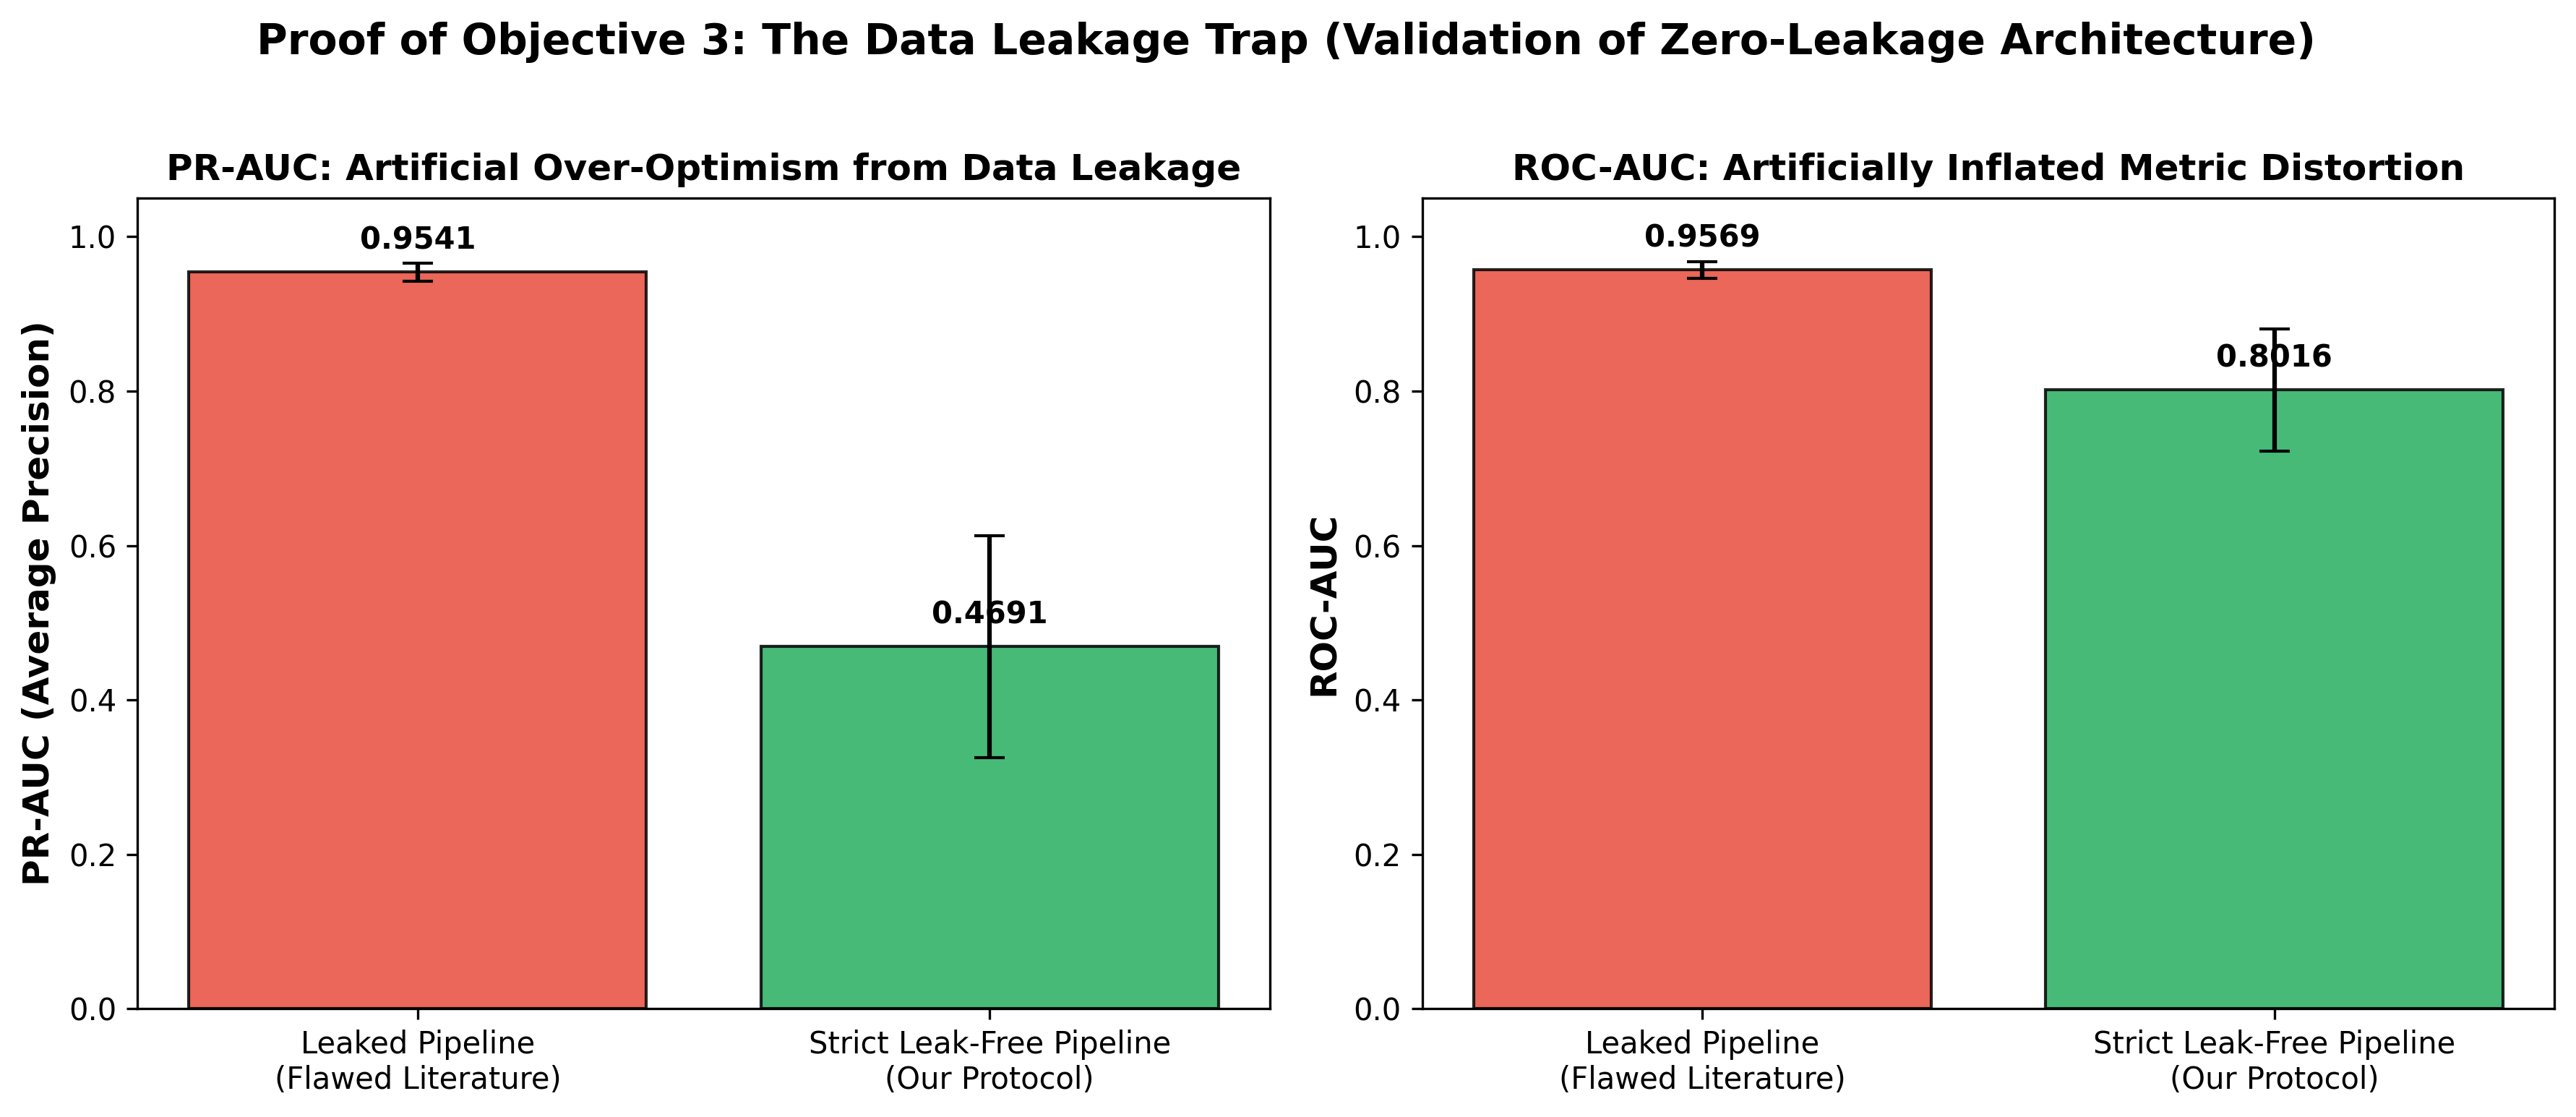
\includegraphics[width=\columnwidth]{figures/fig_leakage.png}
\caption{Separate leakage diagnostic comparing a leaked pipeline with a strict leak-free pipeline. The large metric gap illustrates why splitting must precede resampling; these values are not part of the primary benchmark.}
\label{fig:leakage}
\end{figure}

\begin{figure*}[t]
\centering
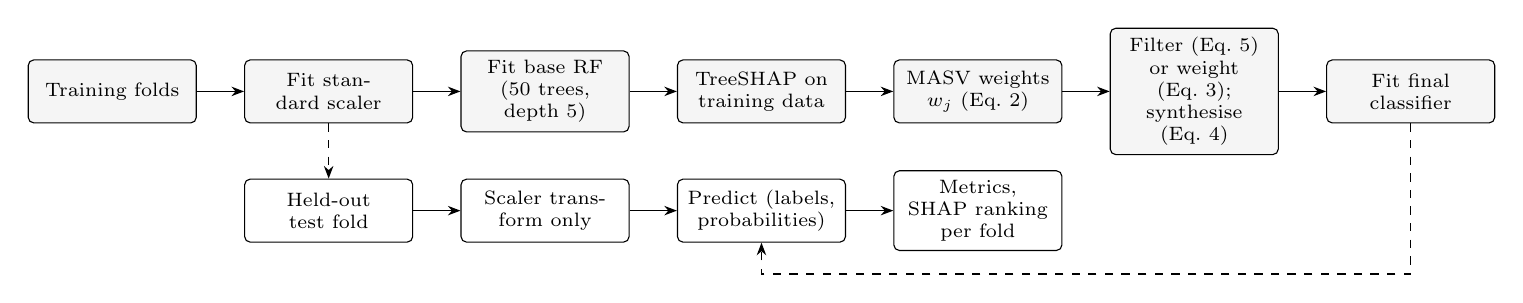
\begin{tikzpicture}[
  node distance=5mm and 6mm,
  box/.style={draw, rounded corners=2pt, align=center, font=\scriptsize, minimum height=8mm, text width=19mm, fill=gray!8},
  tbox/.style={draw, rounded corners=2pt, align=center, font=\scriptsize, minimum height=8mm, text width=19mm, fill=white},
  arr/.style={-{Stealth[length=1.6mm]}, line width=0.5pt}]
\node[box] (tr) {Training folds};
\node[box, right=of tr] (sc) {Fit standard scaler};
\node[box, right=of sc] (rf) {Fit base RF\\(50 trees, depth 5)};
\node[box, right=of rf] (sh) {TreeSHAP on training data};
\node[box, right=of sh] (ma) {MASV weights $w_j$ (Eq.~2)};
\node[box, right=of ma] (sy) {Filter (Eq.~5) or weight (Eq.~3); synthesise (Eq.~4)};
\node[box, right=of sy] (cl) {Fit final classifier};
\node[tbox, below=7mm of sc] (te) {Held-out test fold};
\node[tbox, right=of te] (tt) {Scaler transform only};
\node[tbox, right=of tt] (pr) {Predict (labels, probabilities)};
\node[tbox, right=of pr] (ev) {Metrics, SHAP ranking per fold};
\draw[arr] (tr)--(sc); \draw[arr] (sc)--(rf); \draw[arr] (rf)--(sh); \draw[arr] (sh)--(ma); \draw[arr] (ma)--(sy); \draw[arr] (sy)--(cl);
\draw[arr] (te)--(tt); \draw[arr] (tt)--(pr); \draw[arr] (pr)--(ev);
\draw[arr, dashed] (cl.south) |- ($(pr.south)+(0,-4mm)$) -- (pr.south);
\draw[arr, dashed] (sc.south) -- (te.north);
\end{tikzpicture}
\caption{Per-fold workflow. Every fitted component (scaler, SHAP base estimator, oversampler, classifier) uses training-fold data only; dashed arrows denote transfer of fitted objects to the test fold.}
\label{fig:flow}
\end{figure*}

\subsection{Datasets and preprocessing}
Three binary datasets are used (Table~\ref{tab:data}); the minority class is the less frequent class. The breast-cancer dataset is real; the credit-fraud and NSL-KDD-style datasets are simulations designed to mimic the imbalance and structure of those domains and are not the original datasets. In the credit-fraud simulation, minority samples are shifted by $2.5$ to $4.0$ along seven fixed dimensions with a random sign per sample; consequently, the class means nearly coincide and linear models are difficult to separate by construction. The breast-cancer dataset is the Wisconsin Diagnostic data, with malignant cases subsampled to a 10\% minority ratio. All features are numeric; standardisation is fitted on each training fold. 

\begin{table}[t]
\caption{Benchmark Datasets}
\label{tab:data}
\centering
\small
\begin{tabular}{lcccc}
\toprule
\textbf{Dataset} & \textbf{Samples} & \textbf{Features} & \textbf{IR} & \textbf{Origin} \\
\midrule
Breast cancer & 396 & 30 & 9:1 & Real \\
Credit-fraud sim. & 2000 & 28 & 49:1 & Simulated \\
NSL-KDD-style sim. & 1500 & 35 & 11:1 & Simulated \\
\bottomrule
\end{tabular}
\end{table}

\subsection{Mathematical formulation}
Let $\mathcal{D}=\{(x_i,y_i)\}_{i=1}^{N}$ be a training fold with $x_i\in\mathbb{R}^p$. A base random forest $f_{\text{base}}$ is fitted on $\mathcal{D}$, and TreeSHAP yields the positive-class attribution $\phi_j(x_i)$ of feature $j$ for sample $i$. The mean absolute SHAP value and its normalised form are
\begin{equation}
\mathrm{MASV}_j=\frac{1}{N}\sum_{i=1}^{N}\left|\phi_j(x_i)\right|,
\end{equation}
\begin{equation}
w_j=\frac{\mathrm{MASV}_j}{\sum_{m=1}^{p}\mathrm{MASV}_m},\qquad \sum_{j=1}^{p}w_j=1,
\end{equation}
where $N$ is the number of training samples, $p$ the number of features, and $w_j\ge 0$ the weight of feature $j$ (uniform weights are used if all MASV values vanish). SHAP-Weighted SMOTE replaces the Euclidean metric by
\begin{equation}
d_W(x_a,x_b)=\sqrt{\sum_{j=1}^{p}w_j\,(x_{aj}-x_{bj})^2}.
\end{equation}
Neighbour search with $d_W$ is implemented exactly by Euclidean search on the transformed minority points $x\odot\sqrt{w}$. A synthetic sample is then generated in the original feature space as
\begin{equation}
x_{\text{new}}=x_i+\lambda\,(x_{z}-x_i),\qquad \lambda\sim\mathcal{U}(0,1),
\end{equation}
where $x_i$ is a minority sample, $x_z$ is one of its $k$ nearest minority neighbours under the active metric, and $\lambda$ is drawn independently for each synthetic sample. SHAP-Filtered SMOTE instead ranks features by MASV, sorts the weights in descending order as $w_{(1)}\ge\dots\ge w_{(p)}$, and keeps the smallest subspace whose cumulative weight reaches a threshold $\theta$:
\begin{equation}
p'=\min\Big\{m:\ \sum_{r=1}^{m}w_{(r)}\ge\theta\Big\}.
\end{equation}
Neighbours are searched in the $p'$ retained dimensions with the ordinary Euclidean metric, while interpolation (Eq.~4) uses all $p$ features. The number of synthetic samples is $N_{\text{gen}}=\max(0,N_{\text{maj}}-N_{\text{min}})$, i.e.\ full balancing, with $N_{\text{maj}}$ and $N_{\text{min}}$ the class sizes in the training fold.

\begin{algorithm}[t]
\caption{SHAP-Guided SMOTE (one training fold)}
\label{alg:shap}
\begin{algorithmic}[1]
\REQUIRE $X\in\mathbb{R}^{N\times p}$ (scaled), labels $y$, mode $\in\{$weighted, filtered$\}$, $k$, $\theta$
\ENSURE Resampled $(X',y')$
\STATE Fit $f_{\text{base}}$ on $(X,y)$; compute $\phi_j(x_i)$ with TreeSHAP
\STATE Compute $\mathrm{MASV}_j$ and $w_j$ (Eqs.~1--2)
\STATE $X_{\min}\leftarrow$ minority rows; $N_{\text{gen}}\leftarrow\max(0,N_{\text{maj}}-N_{\text{min}})$
\IF{$N_{\text{gen}}=0$ \OR $N_{\text{min}}<2$} \RETURN $(X,y)$ \ENDIF
\IF{mode = weighted}
  \STATE $Z\leftarrow X_{\min}\odot\sqrt{w}$
\ELSE
  \STATE Select $p'$ features by Eq.~5; $Z\leftarrow X_{\min}[:,\text{selected}]$
\ENDIF
\STATE Find $k'=\min(k,N_{\text{min}}-1)$ nearest neighbours of each row of $Z$
\FOR{$t=1$ \TO $N_{\text{gen}}$}
  \STATE Draw base $i$ uniformly, neighbour $z$ uniformly from its $k'$ neighbours, $\lambda\sim\mathcal{U}(0,1)$
  \STATE $s_t\leftarrow x_i+\lambda(x_z-x_i)$ on $X_{\min}$ (all $p$ features)
\ENDFOR
\RETURN $X'=[X;S]$, $y'=[y;\text{minority label}\times N_{\text{gen}}]$
\end{algorithmic}
\end{algorithm}

\subsection{Implementation and experimental setup}
Methods are implemented in python using scikit-learn, imbalanced-learn~\cite{b18}, the \texttt{shap} package and XGBoost; they comply with the same \texttt{fit\_resample} interface that has been used by the proposed oversamplers. The base estimator is a random forest (50 trees, maximum depth 5). We use $k=5$ and $\theta=0.85$. We evaluate three classifiers with fixed hyperparameters and no tuning: L2 logistic regression (\texttt{liblinear} type, $C=1$), a random forest (100 trees, depth 6, split (min) 4), and XGBoost (100 trees, depth 5, learning rate $0.08$, subsample $0.8$, column sample $0.8$). Random seed with stratified five-fold cross-validation and one repetition is 42. For baselines (no balancing, random oversampling, SMOTE, Borderline-SMOTE, ADASYN, SMOTE-ENN, SMOTE-Tomek), we use library defaults with $k=5$ where applicable and the same fold splits. Running time is measured in wall time with \texttt{perf\_counter} over the full five-fold run of the (sampler, classifier) pair, including the classifier training. All code, configuration and raw result files (CSV and JSON) are available at https://github.com/hasanr-26/SHAP-SMOTE.

\subsection{Evaluation protocol and metrics}
The default decision rule of each classification model (threshold 0.5) is used for predictions. Let $P$ and $R$ be the minority precision and recall. We show: PR-AUC, defined as area under the precision-recall curve $\sum_n (R_n-R_{n-1})P_n$ for all probability thresholds; minority $F1 =2PR/(P+R)$; balanced accuracy, and the expected calibration error with $B=10$ equal-width bins,
\begin{equation}
\mathrm{ECE}=\sum_{b=1}^{B}\frac{|S_b|}{N_{\text{te}}}\,\big|\mathrm{acc}(S_b)-\mathrm{conf}(S_b)\big|,
\end{equation}
where $S_b$ is the set of test samples whose predicted minority probability falls in bin $b$, $N_{\text{te}}$ is the test-fold size, $\mathrm{acc}(S_b)$ the observed minority frequency, and $\mathrm{conf}(S_b)$ the mean predicted probability. Balanced accuracy and the geometric mean are
\begin{equation}
\mathrm{BA}=\tfrac{1}{2}(R_{\text{min}}+R_{\text{maj}}),\qquad \mathrm{G\text{-}mean}=\sqrt{R_{\text{min}}R_{\text{maj}}},
\end{equation}
where $R_{\text{min}}$ and $R_{\text{maj}}$ are the recalls of the minority and majority class. For a feature $j$ with empirical distribution functions $F_j$ (real minority) and $G_j$ (synthetic), the Wasserstein-1 distance and the Kolmogorov--Smirnov statistic are
\begin{equation}
W_1^{(j)}=\int_{-\infty}^{\infty}\left|F_j(t)-G_j(t)\right|dt,\qquad D^{(j)}=\sup_t\left|F_j(t)-G_j(t)\right|,
\end{equation}
and the reported fidelity values are the mean of $W_1^{(j)}$ over features (in the units of the unscaled features) and the fraction of features whose KS test has $p\ge0.05$. For two importance vectors, Kendall's rank correlation is
\begin{equation}
\tau=\frac{n_c-n_d}{p(p-1)/2},
\end{equation}
$P$ is an importance vector in a model, $\mathbf{v}_1$ is an importance vector for an alternative model, and $v_1 \sim \mathcal{N}(\mathbf{0}, \mathbf{I})$ is a random normal vector. Here $n_c$, $n_d$ refer to the number of concordant and discordant feature pairs respectively and $p$ is the number of features; the reported value is the mean over all fold pairs. \emph{Attribution stability} is the mean pairwise Kendall $\tau$ between the global SHAP importance vectors (mean $|\mathrm{SHAP}|$ on the test fold) of the final classifiers obtained in different folds; it thereby characterizes the stability of downstream model explanations. \emph{Fidelity} measures the close similarity of real minority samples to synthetic samples using the empirical $l_1$ Wasserstein metric (average Wasserstein distance per feature) and the fraction of features that pass a two-sample Kolmogorov–Smirnov test at $p\ge 0.05$ (Kolmogorov-Smirnov test). Fidelity is computed once per dataset on the unscaled full data, outside of any cross-validation loop, and is therefore descriptive only. Reported values are means over folds; PR-AUC standard deviations per configuration of Table\ref{tab:cfg}. The previous aggregate table and its figure have been removed because their metrics could not be recalculated for the three-dataset benchmark. 

\section{Results and Discussion}
\subsection{Aggregate comparison}
We found it unsuccessful to combine antecedents from different datasets with different class proportions (balanced-accuracy omitted; see Table~\ref{tab:overall}). There are a few similarities between the primary aggregate summary (the top half of that table) and the lower half of Table~\ref{tab:cfg}: (i) the minority F1 of SMOTE is lower than that of the SHAP-Weighted SMOTE, and (ii) PR-AUC of SMOTE is lower compared to the other methods (SMOTE < SHAP-Weighted SMOTE < SHAP-Filtered SMOTE < 'Unweighted' baseline). These are mutually consistent, qualitative conclusions across the two quantitative summaries.\

Recall from Table~\ref{tab:overall} that the aggregate table from the earlier benchmark is not retained because its calibration, balanced-accuracy, runtime, and fidelity summaries cannot be recomputed reliably from the per-configuration values available in this paper. Table~\ref{tab:cfg} provides the main quantitative comparison for the three remaining sets (nine dataset--classifier configurations).

\textbf{Aggregate calculated from the displayed per-configuration results.} Across the remaining nine configurations, mean PR-AUC is 0.649 for the unbalanced baseline, 0.601 for SMOTE, 0.600 for SHAP-Filtered SMOTE, and 0.609 for SHAP-Weighted SMOTE. For the two methods with F1 values reported for every configuration in Table~\ref{tab:cfg}, mean minority F1 is 0.564 for SMOTE and 0.577 for SHAP-Weighted SMOTE. These are unweighted arithmetic means over configurations, not pooled sample-level metrics. They are descriptive only; no sound significance test was performed.

\textbf{Interpretation.} Using the baseline (unchanged data) is the best of these via the remaining means PR-AUC in the lower half per-configuration table. The F1 of SHAP-Weighted SMOTE > SMOTE in this remaining per-configuration table. This illustrates a trade-off between score ranking and threshold-dependent minority detection. The result does not establish a general advantage for SHAP-guided oversampling.

\subsection{Per-configuration comparison}
Table~\ref{tab:cfg} displays PR-AUC for our imbalanced baseline, SMOTE, and the two proposed methods and F1 for the SMOTE and SHAP-Weighted SMOTE. Four out of nine configurations produced a higher PR-AUC for SHAP-Weighted SMOTE than for SMOTE; in one they were equal, and the inverse for the rest. The biggest gain, that is on NSL-KDD-style XGBoost (+0.042); The biggest loss is on credit-fraud logistic regression (-0.008). In F1, it is higher in six configurations, lower in two, and equal in one. The POD standard deviations on PR-AUC in the result files are usually 0.02 to 0.12 (see Appendix), which amounts to as large or larger than most of the differences between behaviors from configuration to configuration, plus no statistical test was done so we do not claim to be statistically better. 

\begin{table*}[t]
\caption{PR-AUC (Mean $\pm$ SD Over Folds) and F1 (Mean) by Dataset and Classifier for the three-dataset benchmark. LR: Logistic Regression; RF: Random Forest; XGB: XGBoost; BC: Breast Cancer; CF: Credit-Fraud; NSL: NSL-KDD-Style; SHAP-F/W: SHAP-Filtered/Weighted SMOTE}
\label{tab:cfg}
\centering
\small
\begin{tabular}{llcccccc}
\toprule
 & & \multicolumn{4}{c}{\textbf{PR-AUC}} & \multicolumn{2}{c}{\textbf{F1}} \\
\cmidrule(lr){3-6}\cmidrule(lr){7-8}
\textbf{Data} & \textbf{Clf.} & Raw & SMOTE & SHAP-F & SHAP-W & SMOTE & SHAP-W \\
\midrule
BC & LR & .9626$\pm$.027 & .9646$\pm$.031 & .9668$\pm$.031 & .9668$\pm$.031 & .8978 & .9244 \\
BC & RF & .9469$\pm$.048 & .9470$\pm$.037 & .9527$\pm$.028 & .9466$\pm$.042 & .8595 & .8645 \\
BC & XGB & .9552$\pm$.036 & .9485$\pm$.040 & .9455$\pm$.036 & .9485$\pm$.037 & .8730 & .8730 \\
CF & LR & .1736$\pm$.122 & .0915$\pm$.094 & .0853$\pm$.097 & .0832$\pm$.092 & .0683 & .0595 \\
CF & RF & .9708$\pm$.047 & .8756$\pm$.074 & .8762$\pm$.064 & .9040$\pm$.069 & .7686 & .7644 \\
CF & XGB & .9808$\pm$.019 & .9762$\pm$.021 & .9649$\pm$.032 & .9738$\pm$.032 & .8836 & .8994 \\
NSL & LR & .1559$\pm$.018 & .1333$\pm$.011 & .1437$\pm$.022 & .1443$\pm$.016 & .1970 & .2034 \\
NSL & RF & .3273$\pm$.070 & .2154$\pm$.029 & .1982$\pm$.033 & .2115$\pm$.028 & .2455 & .2940 \\
NSL & XGB & .3719$\pm$.063 & .2598$\pm$.040 & .2672$\pm$.042 & .3019$\pm$.064 & .2819 & .3111 \\
\bottomrule
\end{tabular}
\end{table*}



\textbf{Behaviour varying between datasets.} The predictive models are very similar to the simulation on the credit-fraud dataset: using logistic regression for each method (ROC-AUC about 0.50 and PR-AUC below 0.25). The minority shift yields as expected as it was built as the unbalanced baseline, whose PR-AUC is 0.174 and minority recall is only 0.025 (most oversamplers, except for Borderline-SMOTE, lower PR-AUC to around 0.06--0.09). For the NSL-KDD-style simulation, which has classes that overlap, the unbalanced baseline fails for logistic regression and random forest (minority recall 0 F1 0), but oversampling recovers the minority recall; SMOTE outperforms SHAP-Weighted SMOTE under all three configurations of this dataset (+0.006, +0.049, and +0.029). These takeaways reveal that oversampling benefits depend heavily on both the model and data structure.


\subsection{Additional exploratory clinical-dataset figures}
This project also has a additional set of experiments on a Kaggle stroke-prediction dataset. These are shown as exploratory evidence together they are not combined into the three-dataset aggregate or the per-configuration table above. The plots were produced in separate experimental runs and with different comparison sets -- one thus cannot rely on their numerical values to complement information found in the primary benchmark, but rather interpret the numerical values in each figure.

Figure~\ref{fig:stroke-weighting} shows the comparison of four feature-weighting paradigms of one run on this stroke-dataset. F1 is 0.2177 and ECE 0.1857 for TreeSHAP MASV weighting  while Euclidean SMOTE Has F1 0.2326 and ECE 0.2234. Its PR-AUC is 0.1434 versus 0.1548 for Euclidean SMOTE. Thus this run resulted in TreeSHAP MASV weighting having a lower reported calibration error but not on PR-AUC or minority F1. 

\begin{figure*}[t]
\centering
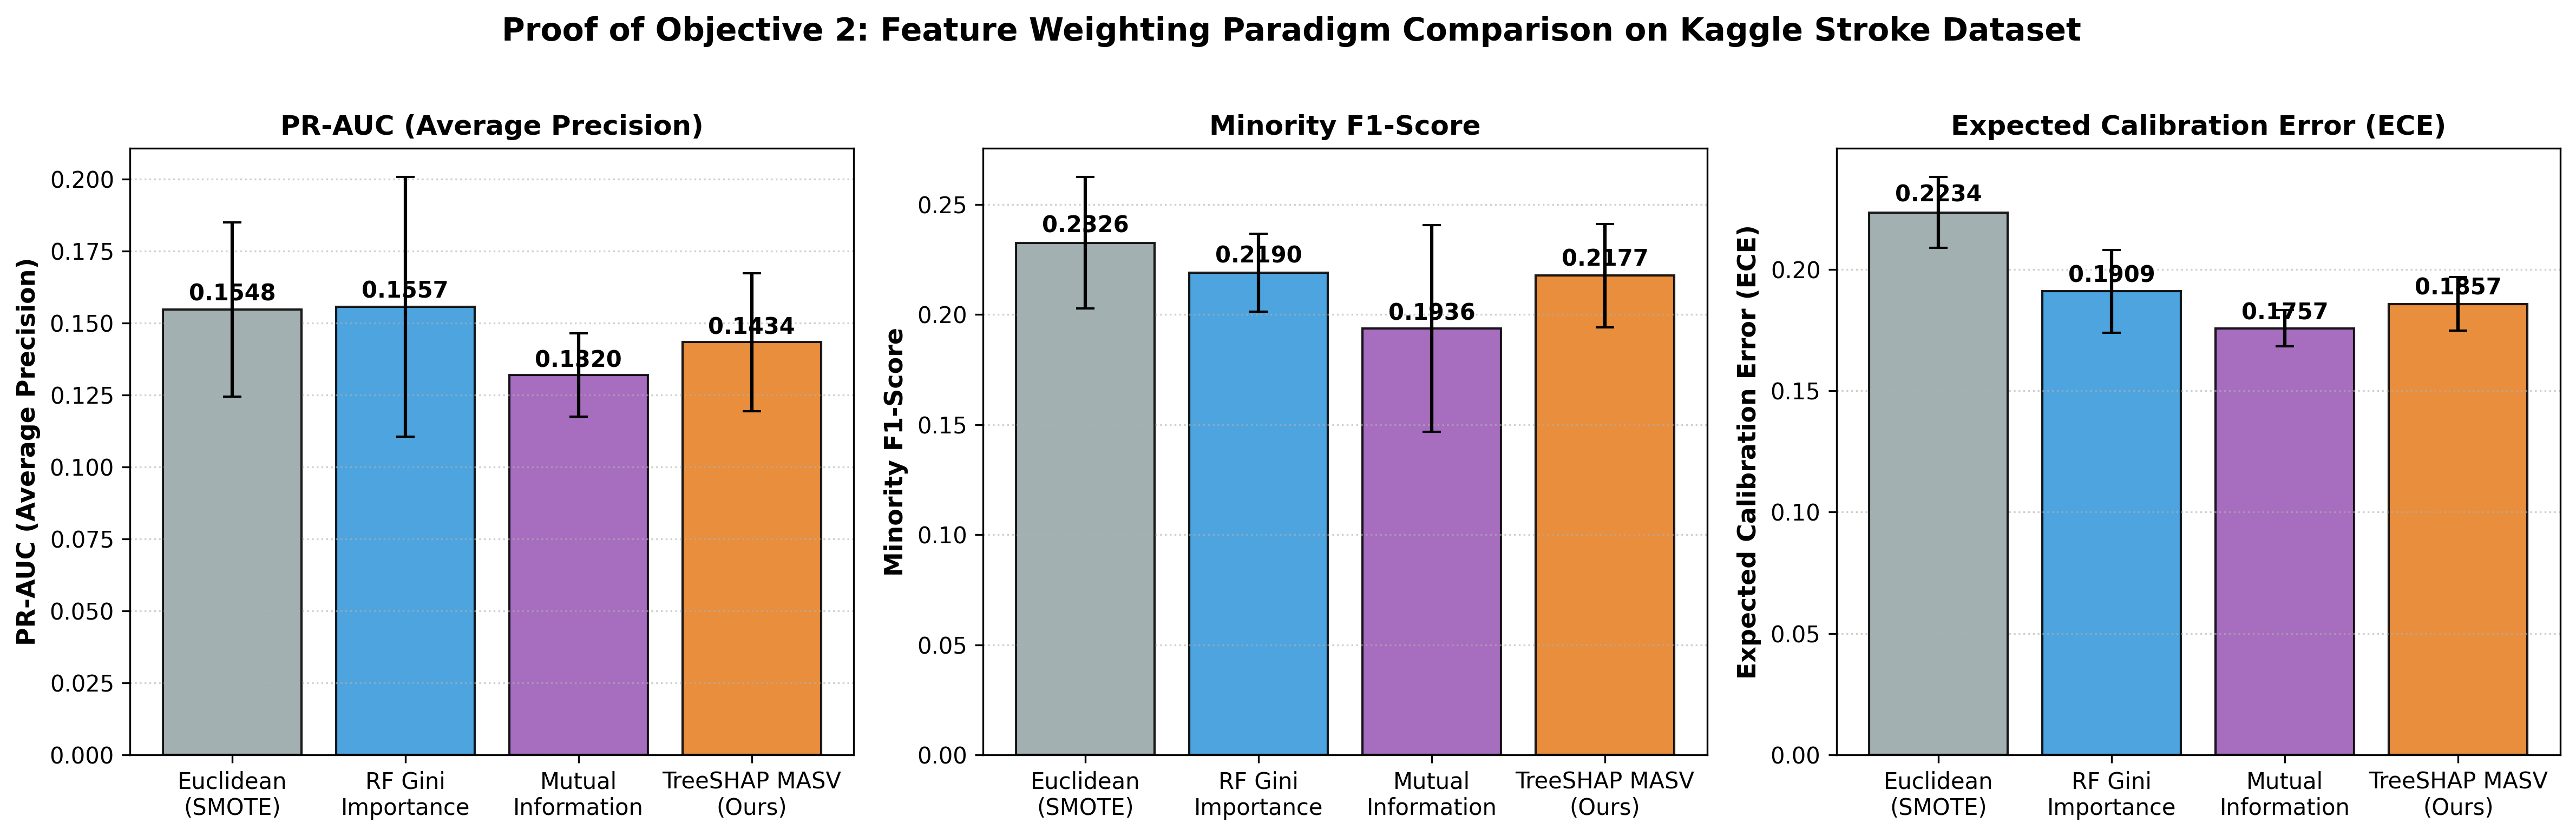
\includegraphics[width=0.98\textwidth]{figures/fig_stroke_weighting.png}
\caption{Exploratory comparison of feature-weighting paradigms on the Kaggle stroke dataset. These values belong to a separate run and are not included in the main benchmark aggregates.}
\label{fig:stroke-weighting}
\end{figure*}

Figure~\ref{fig:stroke-pr-calibration} presents precision--recall and probability-calibration curves from another clinical-dataset run. The reported average precision values are 0.160 for the raw baseline, 0.140 for standard SMOTE, 0.140 for Borderline-SMOTE, 0.126 for SHAP-Filtered SMOTE, and 0.130 for SHAP-Weighted MASV-SMOTE. In this plot, the unbalanced model has the highest average precision. The reliability diagram also shows deviations from the ideal diagonal, so resampling should not be assumed to improve probability calibration.

\begin{figure*}[t]
\centering
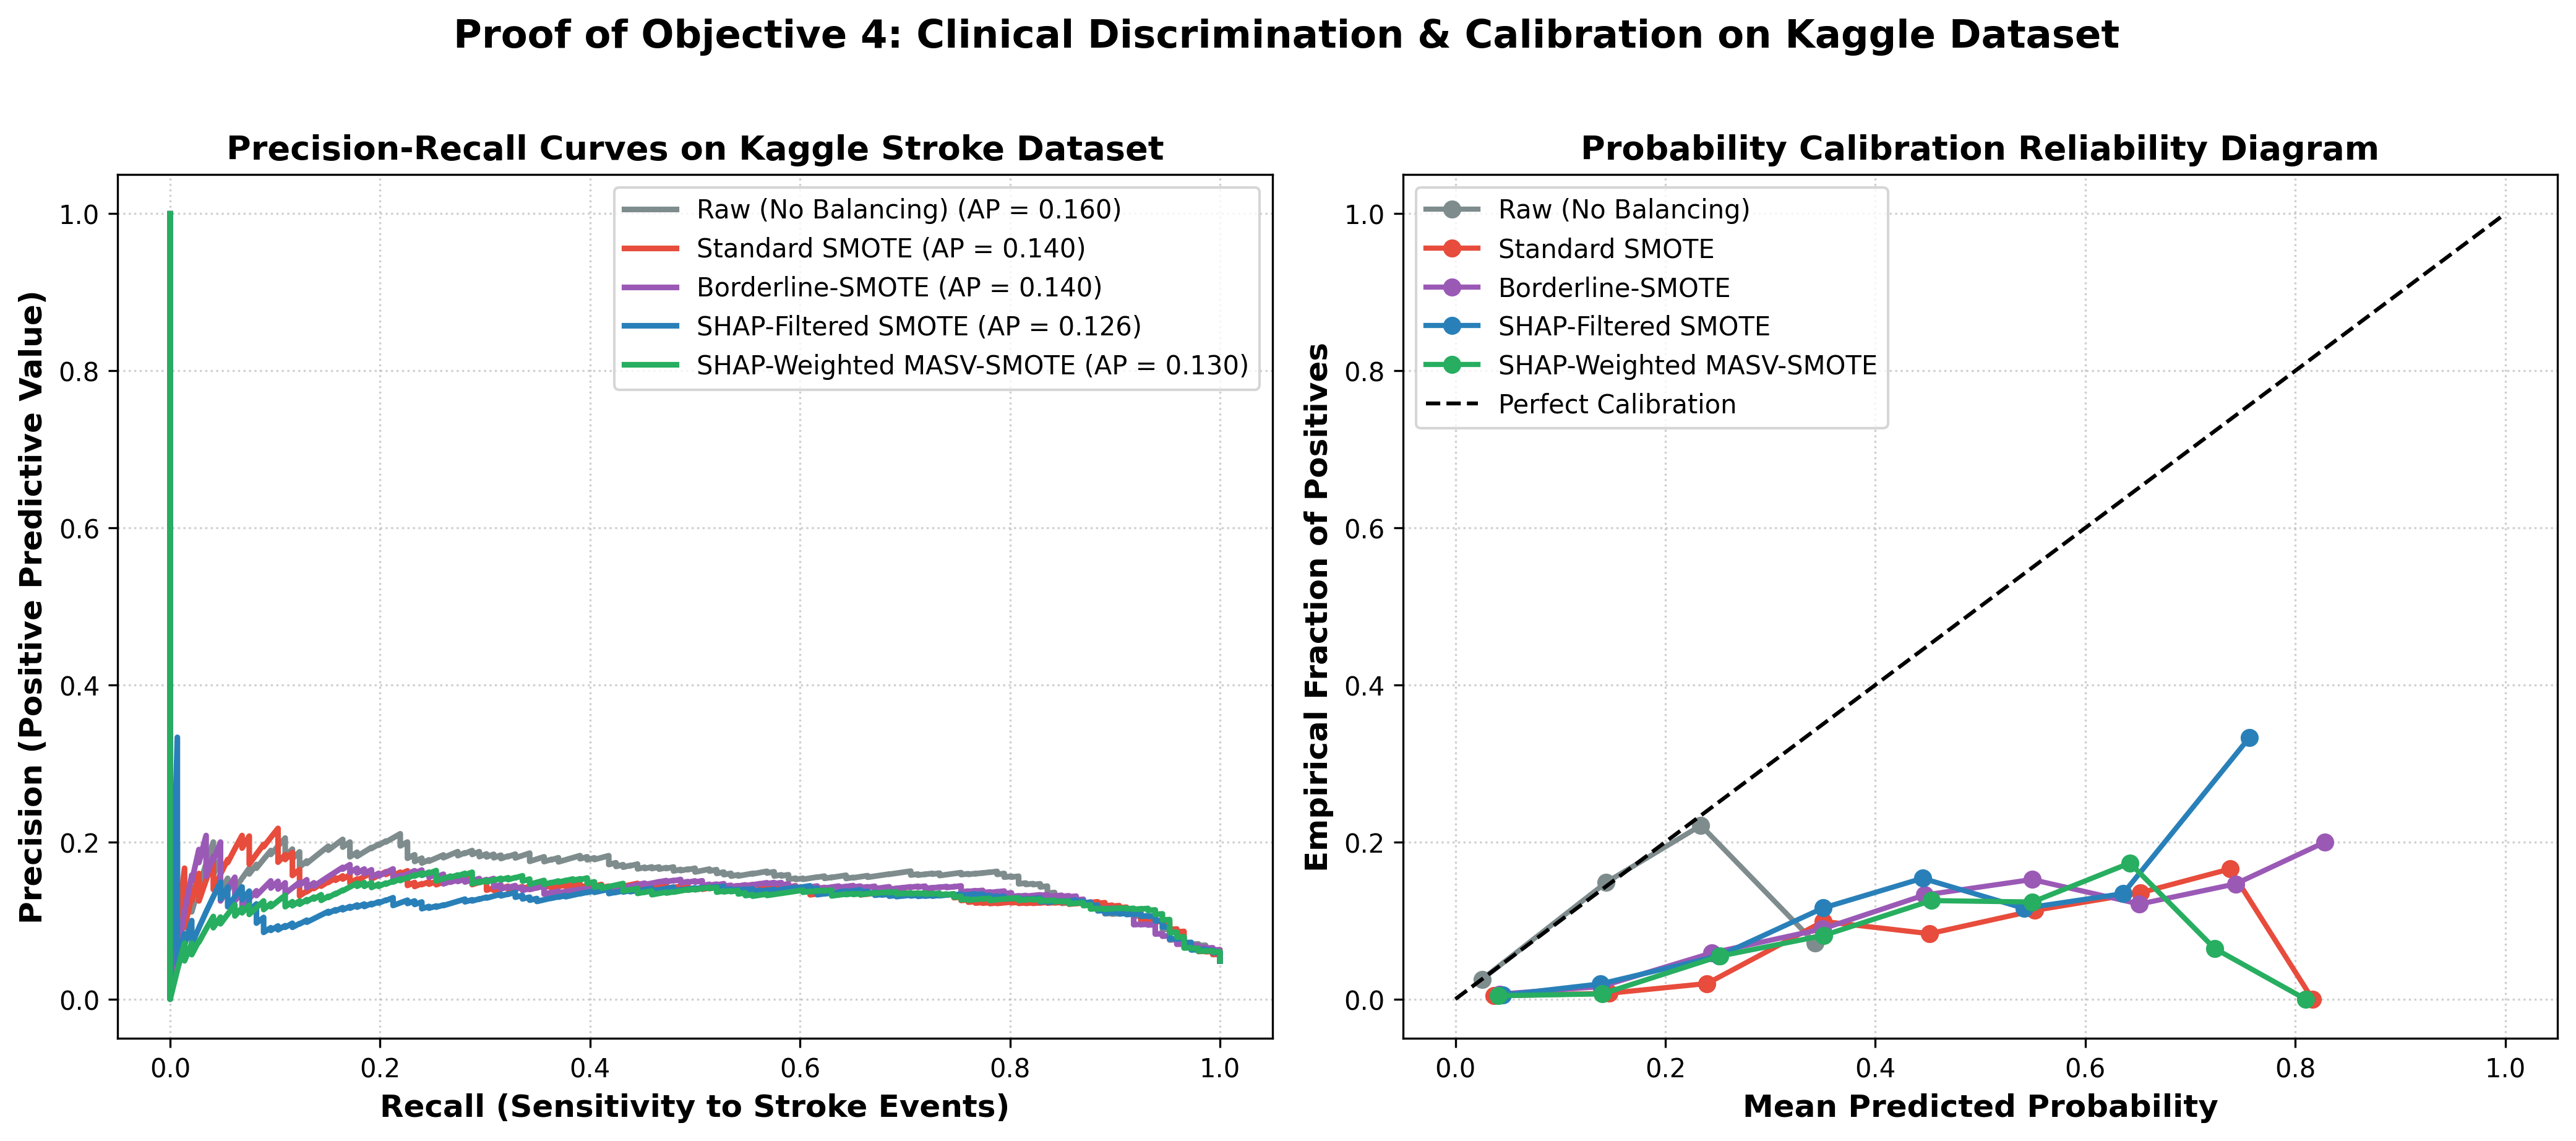
\includegraphics[width=0.98\textwidth]{figures/fig_stroke_pr_calibration.png}
\caption{Precision--recall curves and a reliability diagram for a separate Kaggle stroke-dataset run. Average precision is shown in the legend; these values are not combined with the primary benchmark.}
\label{fig:stroke-pr-calibration}
\end{figure*}

A further five-fold analysis reports a paired Wilcoxon $p$-value of 0.3125 for cross-fold PR-AUC dispersion (Fig.~\ref{fig:stroke-significance}). This does not provide evidence of a statistically significant difference at the conventional level of 0.05. The figure also reports mean (pairwise Kendall) stability values of $0.833$ for the raw baseline, $0.848$ for standard SMOTE, $0.791$ for Borderline-SMOTE, $0.720$ for SHAP-Filtered SMOTE, and $0.837$ for SHAP-Weighted MASV-SMOTE. In this run, the SHAP-filtered method has the lowest displayed attribution stability; the weighted method is close to, but slightly below, the standard SMOTE. These values are specific to this exploratory run and should not be directly compared against the random-forest analysis in Table~\ref{tab:tau} of the primary benchmark. 

\begin{figure*}[t]
\centering
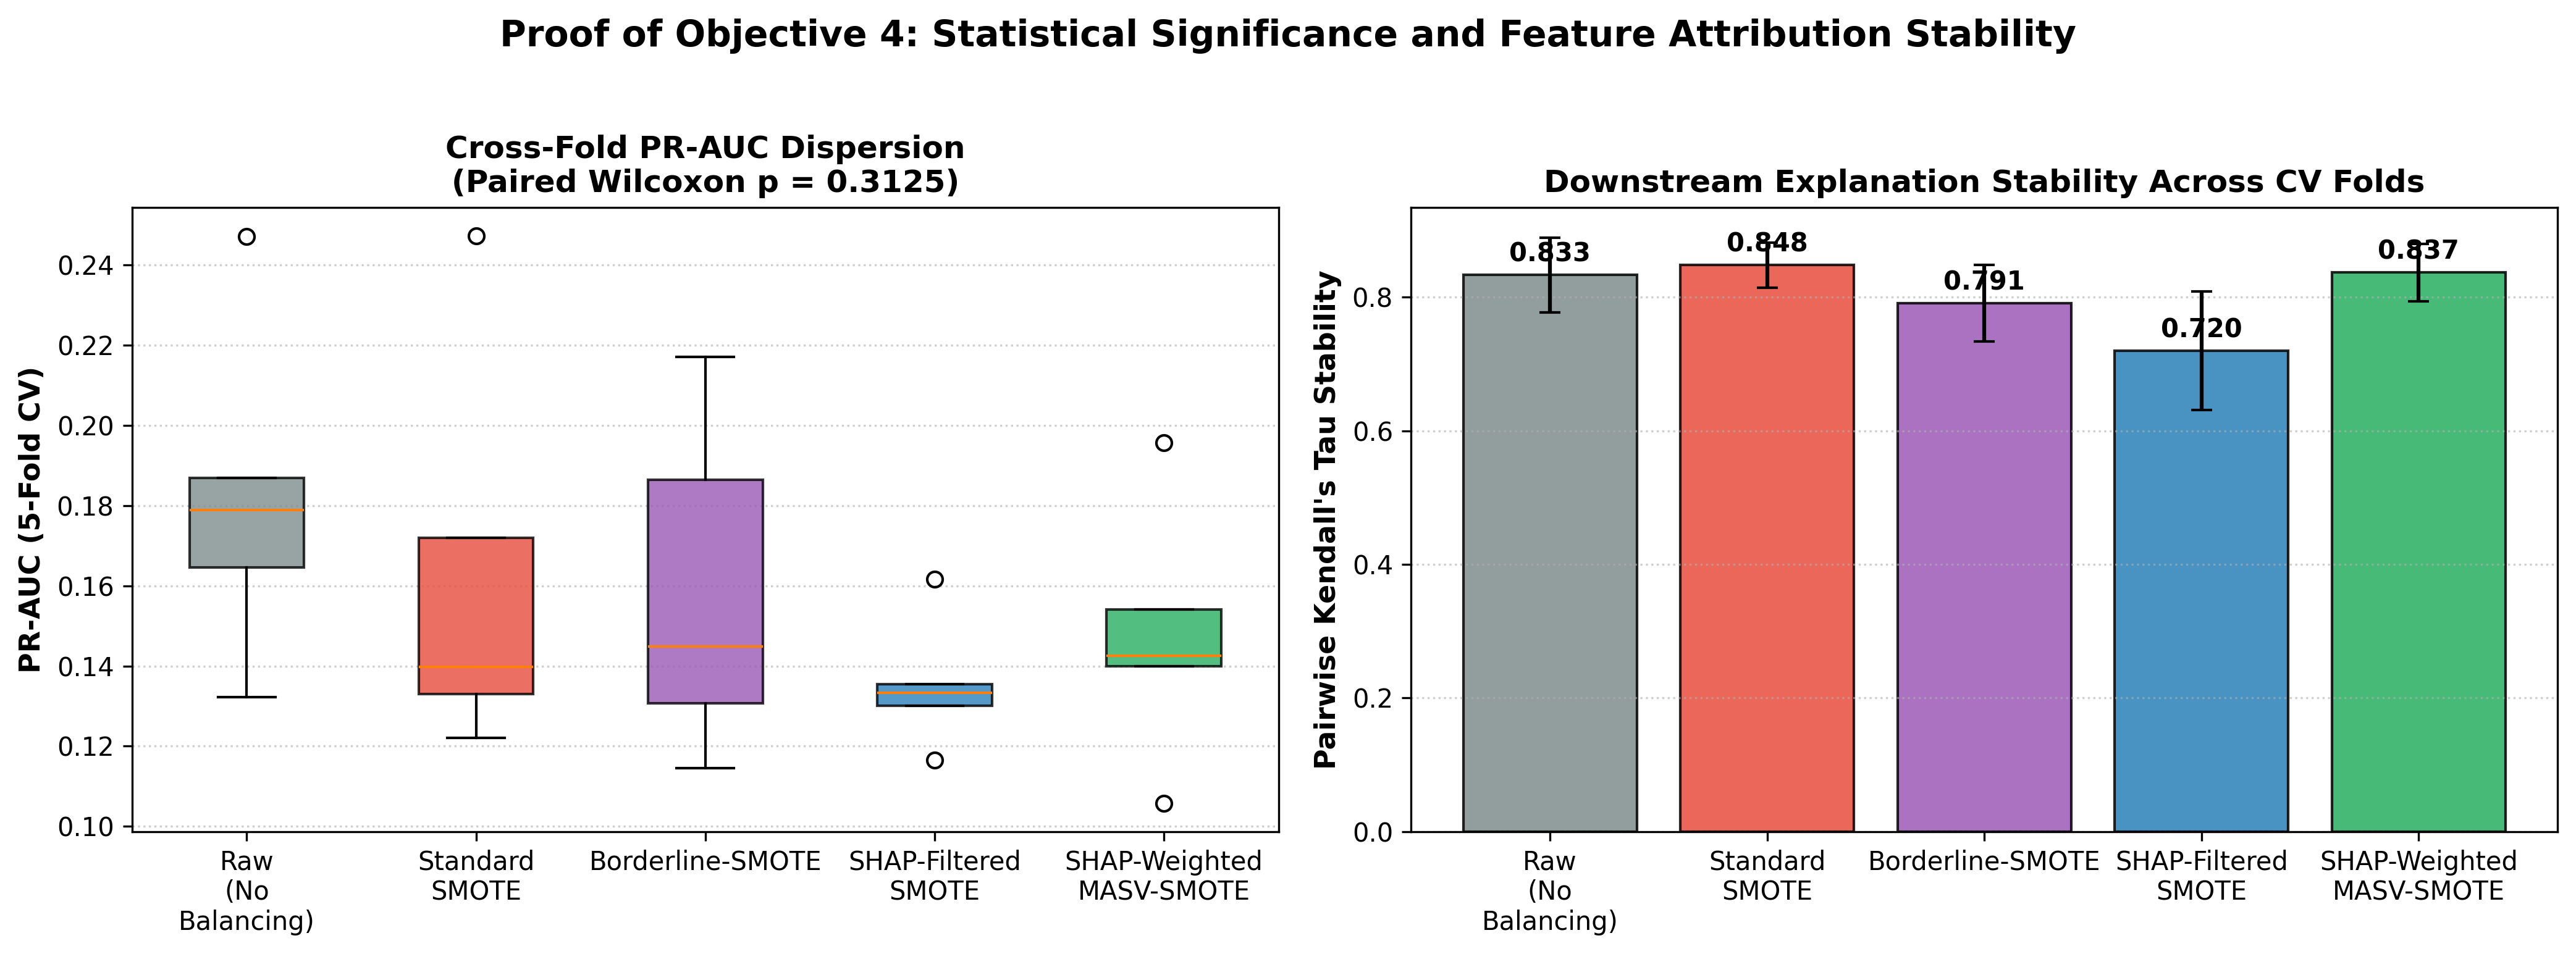
\includegraphics[width=0.98\textwidth]{figures/fig_stroke_significance_stability.png}
\caption{Exploratory five-fold PR-AUC dispersion and downstream attribution stability on the clinical dataset. The paired Wilcoxon result is $p=0.3125$; the displayed analysis does not establish a significant difference.}
\label{fig:stroke-significance}
\end{figure*}

\subsection{Relation to published studies}
For the cross-examination with published outcomes: \cite{b7} and \cite{b8} differed generally from us in datasets, procedures, and metrics; K-IPO~\cite{b8} evaluates the preservation of the original data's importance ranking, which we did not measure (instead we measure consistency across training splits training the model's explanations). It is necessarily qualitative: the dataset-dependency on the benefits that we see is in line with the conclusion of~\cite{b3} that the overlap and noise of a given oversampler, rather than imbalance ratio itself, determine its effectiveness but our experiments do not examine that hypothesis directly.

\subsection{Attribution stability}
Table~\ref{tab:tau} reports the mean pairwise Kendall $\tau$ between fold-wise SHAP importance rankings of the final random-forest classifiers. Values range from 0.503 to 0.758 across the three remaining datasets. The SHAP-guided variants are not consistently more stable than SMOTE: SHAP-Weighted SMOTE is higher on credit-fraud (0.614 vs 0.606) and lower on breast cancer (0.752 vs 0.758) and NSL-KDD-style data (0.577 vs 0.602). SHAP-Filtered SMOTE is lower than SMOTE on credit-fraud and NSL-KDD-style data, and slightly lower on breast cancer. We therefore cannot conclude that attribution-guided oversampling stabilises downstream explanations. \textbf{An implementation defect affects this analysis:} for XGBoost the attribution step failed silently inside an exception handler, and the stored $\tau$ is 0.0 in every XGBoost row. These values are not measurements and are excluded from Table~\ref{tab:tau}; they also deflate any average that includes XGBoost, which is why we do not report a global stability mean.

\begin{table}[t]
\caption{Kendall $\tau$ Attribution Stability, Random Forest Only}
\label{tab:tau}
\centering
\small
\begin{tabular}{lccc}
\toprule
\textbf{Method} & \textbf{BC} & \textbf{CF} & \textbf{NSL} \\
\midrule
Raw & 0.745 & 0.580 & 0.507 \\
SMOTE & 0.758 & 0.606 & 0.602 \\
SHAP-Filtered & 0.756 & 0.600 & 0.503 \\
SHAP-Weighted & 0.752 & 0.614 & 0.577 \\
\bottomrule
\end{tabular}
\end{table}

\subsection{Runtime and implementation observations}
During a before-and-after study with a fast 50 ms SHAP instance in the 155 experiments, the mentioned four-dataset run took approximately 3.70 to 3.74 seconds for the SHAP-guided methods and 2.11 secs for SMOTE. These timings are just historical implementation numbers and are not re-executed three-dataset benchmark results. The 3-dataset benchmark should be re-run for a correct runtime comparison.

\subsection{Observations on baselines}
SMOTE-Tomek produced the same results as SMOTE to four decimal places across all configurations. This indicates that removing Tomek links had no measurable effect under the settings tested. Since we did not examine this finding further, we treat SMOTE-Tomek as equivalent to SMOTE in this study.

\section{Complexity Analysis}
Let $N$ be the training-fold size, $p$ the number of features, $T$ the number of trees of the base forest, $D$ its maximum depth, $L$ the maximum number of leaves per tree, $N_{\text{min}}$ the minority size, and $N_{\text{gen}}$ the number of synthetic samples. For the base forest's training phase, we use other than the 50\% top features “balanced-tree” assumption on average; $O(T,p,N\log N)$. Running Exact TreeSHAP on all $N$ training samples requires $O(N,T,L,D^2)$~\cite{b6}. Further, MASV and weight calculation cost $O(Np)$ in addition. The brute-force neighbor search of minority points is $O(N_{\text{min}}^2,p)$ or $O(N_{\text{min}}\log N_{\text{min}}\cdot p)$ when a tree-based index performs well in low dimension; for SHAP-Filtered SMOTE, replace $p$ with $p'\le p $. To compute the synthetic samples takes time $O(N_{\text{gen}},p)$ with storage $O((N+N_{\text{gen}}),p)$. Increased computational cost is incurred by offering an at possible cost — or "boot cost," which is used in your iterative A1A full run. The overhead of the base-model fit and TreeSHAP term dominates the asymptotic cost "beyond" SMOTE, as the attribution cost is paid per training fold and is independent of $N_{\text{gen}}$. On this three-dataset benchmark, we did not report runtime ratio because no timing measures are available for this dataset set (the available timing estimates were not re- computed).

\section{Limitations}
Limitations The study has the following limitations. (i) Of these three datasets, two are simulations and only one is genuine, which limits the extent to which the findings can be applied to real-world data. (ii) There was one repetition of five-fold cross-validation with a fixed seed, no hyperparameter tuning, and no significance tests. (iii) The attribution-stability measure is invalid for XGBoost because of the silent failure noted above. (iv) In the original experiment, fidelity was computed on unscaled data outside of the cross-validation loop, and a recomputed aggregate is therefore not reported here. (v) The study was only concerned with binary operands; categorical encoding and mixed-type distances remained untested. (vi) A fixed threshold of 0.5 for F1, precision, and recall was used To avoid probability recalibration on the oversampled models. (vii) Different problems (with very different degrees of difficulty) were mixed when calculating averages across datasets. (viii) Experiments were performed on the default dataset sizes, which differ from those in the accompanying configuration file; the values in Table~\ref{tab:data} are those of the latter, and indeed of the former. 

\section{Conclusion and Future Scope}
We proposed SHAP-Filtered and SHAP-Weighted SMOTE (which get neighbourhoods from mean absolute SHAP values computed inside each training fold) and benchmarked them against classical baselines on three datasets and three classifiers in a leakage-aware protocol. The mean minority F1 of SHAP-Weighted SMOTE is 0.577 vs 0.564 for SMOTE, and the mean PR-AUC is 0.609 vs 0.601 for SMOTE. Besides that, in the rest the highest mean PR-AUC (0.649) is achieved by the imbalanced baseline, as illustrated in the per-configuration table. In addition, no significant tests were run for the annotation stability of SHAP-guided methods, nor did they consistently improve attribution stability. This study attempts to provide partial solutions for objectives O2--O4: the methods are implemented and evaluated, but the study does not show a clear advantage in terms of the benefits over classical oversampling techniques on these data.

Future work: (i) reconcile the exploratory clinical stroke-dataset runs with a single documented protocol, then evaluate that dataset with repeated cross-validation and appropriate significance tests; (ii) fix the XGBoost attribution step and report stability for all classifiers; (iv) move fidelity analysis inside the folds on scaled data; (iv) add the post-generation validation touchpoint (T4) and Kendall-type constraints as in~\cite{b8}; (v) extend the metric weighting to mixed categorical and numeric features; and (vi) consider probability calibration after oversampling.

\begin{thebibliography}{00}
\bibitem{b1} W. Chen, K. Yang, Z. Yu, Y. Shi, and C. L. P. Chen, ``A survey on imbalanced learning: Latest research, applications and future directions,'' \emph{Artif. Intell. Rev.}, vol. 57, art. no. 137, 2024, doi: 10.1007/s10462-024-10759-6.
\bibitem{b2} N. V. Chawla, K. W. Bowyer, L. O. Hall, and W. P. Kegelmeyer, ``SMOTE: Synthetic minority over-sampling technique,'' \emph{J. Artif. Intell. Res.}, vol. 16, pp. 321--357, 2002.
\bibitem{b3} A. Fern\'andez, S. Garc\'ia, F. Herrera, and N. V. Chawla, ``SMOTE for learning from imbalanced data: Progress and challenges, marking the 15-year anniversary,'' \emph{J. Artif. Intell. Res.}, vol. 61, pp. 863--905, 2018, doi: 10.1613/jair.1.11192.
\bibitem{b4} D. Elreedy and A. F. Atiya, ``A comprehensive analysis of synthetic minority oversampling technique (SMOTE) for handling class imbalance,'' \emph{Inf. Sci.}, vol. 505, pp. 32--64, 2019.
\bibitem{b5} S. M. Lundberg and S.-I. Lee, ``A unified approach to interpreting model predictions,'' in \emph{Proc. Adv. Neural Inf. Process. Syst. (NeurIPS)}, vol. 30, 2017.
\bibitem{b6} S. M. Lundberg \emph{et al.}, ``From local explanations to global understanding with explainable AI for trees,'' \emph{Nat. Mach. Intell.}, vol. 2, no. 1, pp. 56--67, 2020.
\bibitem{b7} T. Ahmad and R. M. Ijtihadie, ``SHAP-based feature selection and MASV-weighted SMOTE for enhanced intrusion detection,'' Institut Teknologi Sepuluh Nopember, Surabaya, Indonesia..
\bibitem{b8} M. Tyrovolas \emph{et al.}, ``K-IPO: Kendall-constrained importance preserving oversampling for imbalanced tabular data,'' arXiv:2607.16478, 2026.
\bibitem{b9} M. S. Santos, J. P. Soares, P. H. Abreu, H. Araujo, and J. Santos, ``Cross-validation for imbalanced datasets: Avoiding overoptimistic and overfitting approaches,'' \emph{IEEE Comput. Intell. Mag.}, vol. 13, no. 4, pp. 59--76, Nov. 2018.
\bibitem{b10} T. Saito and M. Rehmsmeier, ``The precision-recall plot is more informative than the ROC plot when evaluating binary classifiers on imbalanced datasets,'' \emph{PLoS ONE}, vol. 10, no. 3, art. e0118432, 2015, doi: 10.1371/journal.pone.0118432.
\bibitem{b11} H. He and E. A. Garcia, ``Learning from imbalanced data,'' \emph{IEEE Trans. Knowl. Data Eng.}, vol. 21, no. 9, pp. 1263--1284, Sep. 2009.
\bibitem{b12} H. Han, W.-Y. Wang, and B.-H. Mao, ``Borderline-SMOTE: A new over-sampling method in imbalanced data sets learning,'' in \emph{Advances in Intelligent Computing (ICIC)}, LNCS vol. 3644, Springer, 2005, pp. 878--887.
\bibitem{b13} H. He, Y. Bai, E. A. Garcia, and S. Li, ``ADASYN: Adaptive synthetic sampling approach for imbalanced learning,'' in \emph{Proc. IEEE Int. Joint Conf. Neural Netw. (IJCNN)}, 2008, pp. 1322--1328.
\bibitem{b14} G. E. A. P. A. Batista, R. C. Prati, and M. C. Monard, ``A study of the behavior of several methods for balancing machine learning training data,'' \emph{ACM SIGKDD Explor. Newsl.}, vol. 6, no. 1, pp. 20--29, 2004.
\bibitem{b15} G. Douzas, F. Bacao, and F. Last, ``Improving imbalanced learning through a heuristic oversampling method based on k-means and SMOTE,'' \emph{Inf. Sci.}, vol. 465, pp. 1--20, 2018, doi: 10.1016/j.ins.2018.06.056.
\bibitem{b16} G. Douzas and F. Bacao, ``Geometric SMOTE: A geometrically enhanced drop-in replacement for SMOTE,'' \emph{Inf. Sci.}, vol. 501, pp. 118--135, 2019, doi: 10.1016/j.ins.2019.06.007.
\bibitem{b17} M. A. Walauskis \emph{et al.}, ``SHAP-based feature selection for enhanced unsupervised labeling,'' \emph{IEEE Access}, 2025..
\bibitem{b18} G. Lema\^itre, F. Nogueira, and C. K. Aridas, ``Imbalanced-learn: A Python toolbox to tackle the curse of imbalanced datasets in machine learning,'' \emph{J. Mach. Learn. Res.}, vol. 18, no. 17, pp. 1--5, 2017.
\end{thebibliography}

\end{document}
